\mysubsubsection{Onboarding Problems}
$25\%$ of the people reported that lack of proper documentation is the biggest problem they faced while contributing to open source projects. This makes the joining process very time consuming, which trigger delays before the very first contribution can actually be done. When a project involves software development,  having an up and running installation to tinker with is an another important onboarding issue. Some respondents ($19\%$) contributing to technical open source projects reported that they had troubles with installing and running the software on their machines. In spite of the availability of the documentation, they could not find a solution to their problems. The responses to their mails are very cryptic and are mostly stuck with solving the problem on their own, resulting in wastage of time. Similar to this issue is the high complexity of the code base which required lot of time to even understand the project. Because of this it has been hard to get up to speed and make a contribution to a current need or issue in the project.

\begin{figure}[ht!]
\centering
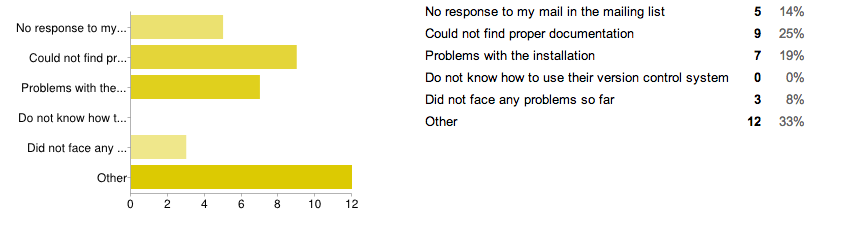
\includegraphics[width=130mm]{chapters/img/problems_faced.png}
\caption{Problems faced by new contributors. {\bf Can you say more about Other ?}}
\label{fig:problem_faced}
\end{figure}

Another major problem reported is the lack of sense of community in the open source projects respondents wanted to join (\todo{does it come from other in Figure \ref{fig:problem_faced}}). Some complained that they did not get any response or favorable warm response if at all, to their introduction mail in the mailing list. This led to a sense of alienation and fear of contribution by the newbies \todo{do we have any example of someone having left a project because of this?}. 

{\bf [should be in the Discussion ?] A standard, proper, detailed documentation  would help overcome onboarding problems. One of the reasons could be  that many open source projects have multiple platforms for members to communicate with each other - forums, the wiki, the mailing lists, and the issue tracker. However, all of these are separate systems with their own login info and digging into these huge mines and getting required information seems to be a major obstacle. If all the important information like ``Where to start and How to contribute to the project" and ``trouble shooting areas" from these systems had been put in single place, the newbie would have found it easier to take his first steps in the journey of open source contribution. Indeed, some of the members of this class are contributing in making documentation more comprehensive and organized \todo{who? evidence from survey ?}.}





